%===============================================================================
% Autoři: Michal Bidlo, Bohuslav Křena, Jaroslav Dytrych, Petr Veigend a Adam Herout 2018
\chapter{Úvod}
Cieľom tejto práce je poskytnúť čitateľovi rýchly prehľad v problematike optických aberácii.
Ich znalosť môže čitateľovi pomôcť pri tvorbe realistických vykreslovacích programov alebo
pri zaujímavých filtroch obrazu. Vzhľadom na komplexnosť týchto javov poskytuje text značne 
zjednodušený popis a pre precíznu znalosť je vhodné vyhľadať doporučenú literatúru, napr. knihu pána
Hechta\cite{hechtoptics}.
%Aproximácie, ktoré ako inžinieri používame, nám často zjednodušujú prácu, no zároveň nám pília konár
%pod nohami v prípadoch, keď vyžadujeme neomylnosť a presnosť.
%Obdobná situácia sa vyskytuje aj v optike. Aberácie predstavujú odchýlky, ktoré vznikajú zjedošením
%modelu optických systémov. Ich nesprávne pochope, či dokonca ignorácia, môže viesť k fatálnym chybám
%ako napríklad v prípade Hubblového vesmírneho teleskopu.

\section{Aberácie}
Podľa literatúry je aberácia definovaná ako \textit{odchíľka od idealizovaného modelu Gaussovej
optiky}\cite{hechtoptics}, či \textit{neschopnosť optického systému zaostriť ľúče do jedného bodu}[Wikipédia].

V praxi sú aberácie kolekcia javov, ktoré nastávajú v optických systémoch, a ktorých prítomnosť
obvykle nie je žiadúca. Nakoľko táto práca vznikla na pôde fakulty informačných technológii, budú
nás v tom texte zaujímať negatívne javy, ktoré vznikajú v obraze pri výskyte týchto aberácii.

Aberácie prestavujú odchýlky od ideálneho optického modelu, ktoré sa v ňom nevyskytujú z dôvodu
zjednodušenia formalizov oproti reálnym optickým systémom. Príkladom je \textit{Snellov zákon},
ktorého zjednodušená forma popisuje lom svetla len pre tzv. paraxiálne uhly. \cite{hechtoptics}.

Dôsledkom aberácii sú \textit{optické vady}, ktoré sa prejavujú rozmazaním alebo deformáciou obrazu. V praxi sa tieto
vady riešia rozšírením optickej sústavy o ďalšie prvky, ktoré korigujú ľúče, prípadne pomocou
špecializovaného software-u \cite{automaticRemovalCA}. Softwareové riešenie ale nemusí byť vždy žiaduce nakoľko nemusí
byť fyzikálne presné a môže sa jednať o istú aproximáciu.

Počiatok skúmania aberácii siaha ku matematikovi \textbf{Ludwigovi von Seidelovi} (1821-1896), ktorý
pôsobil na bavorských univerzitách a ktorého jednou z oblastí záujmu bola astronómia. \cite{seidel}
Podstatným krokom pána Seidela bolo zadefinovanie piatich koeficientov v rovnici, ktorá definuje
prechod paprskov šošovkou z pohľadu optiky vyššieho rádu. Vhodnou voľbou týchto koeficientov je 
možné získať predpis hlavných geometrických aberácii. Táto rovnica bola pomenovaná podľa neho a 
v literatúre je označovaná ako \textit{Seidler sums}.

K skúmaniu aberácii ešte skorej prispel aj \textbf{Isaac Newton}, ktorý sa venoval ľudskému vnímaniu svetla a
popísal jav \textit{disperzie svetla} na hranole, ktorá sa týka \textit{chromatickej aberácie}. \cite{elert}

\section{Monochromatické aberácie}
Monochromatické aberácie predstavujú odchýlky, ktoré sa vyskytujú už pri jednej vlnovej dĺžke.
\subsection{Sférická aberacia}
Sférická aberácia nastáva pri dopade rovnobežných ľúčov na sférický optický prvok, ktorým môže byť
šošovka, či zrkadlo. 
Podľa ideálneho modelu šošovky by sa pri dopade na rozhranie zakrivenej šošovky mal ľúč lámať do ohniska šošovky, ktoré
je dané polomerom krivosti danej šošovky. V praxi sa vplyvom zakrivenia lúč lámu do rôznych
ohniskových bodov \cite{elisa}[str. 12]. Platí, že lúč, ktorý je vzdialenejší od optickej osy, pretne optickú os bližšie
ku rovine optického prvku. Táto situácia je zachytená na obrázku \ref{saill}.

Dôsledkom tohoto javu je rozmazanie obrazu. Bodové predmety sa preto javia ako kruhy s postupným
prechodom od stredu zobrazenia bodu.

\begin{figure}[h]
\centering
\label{saill}
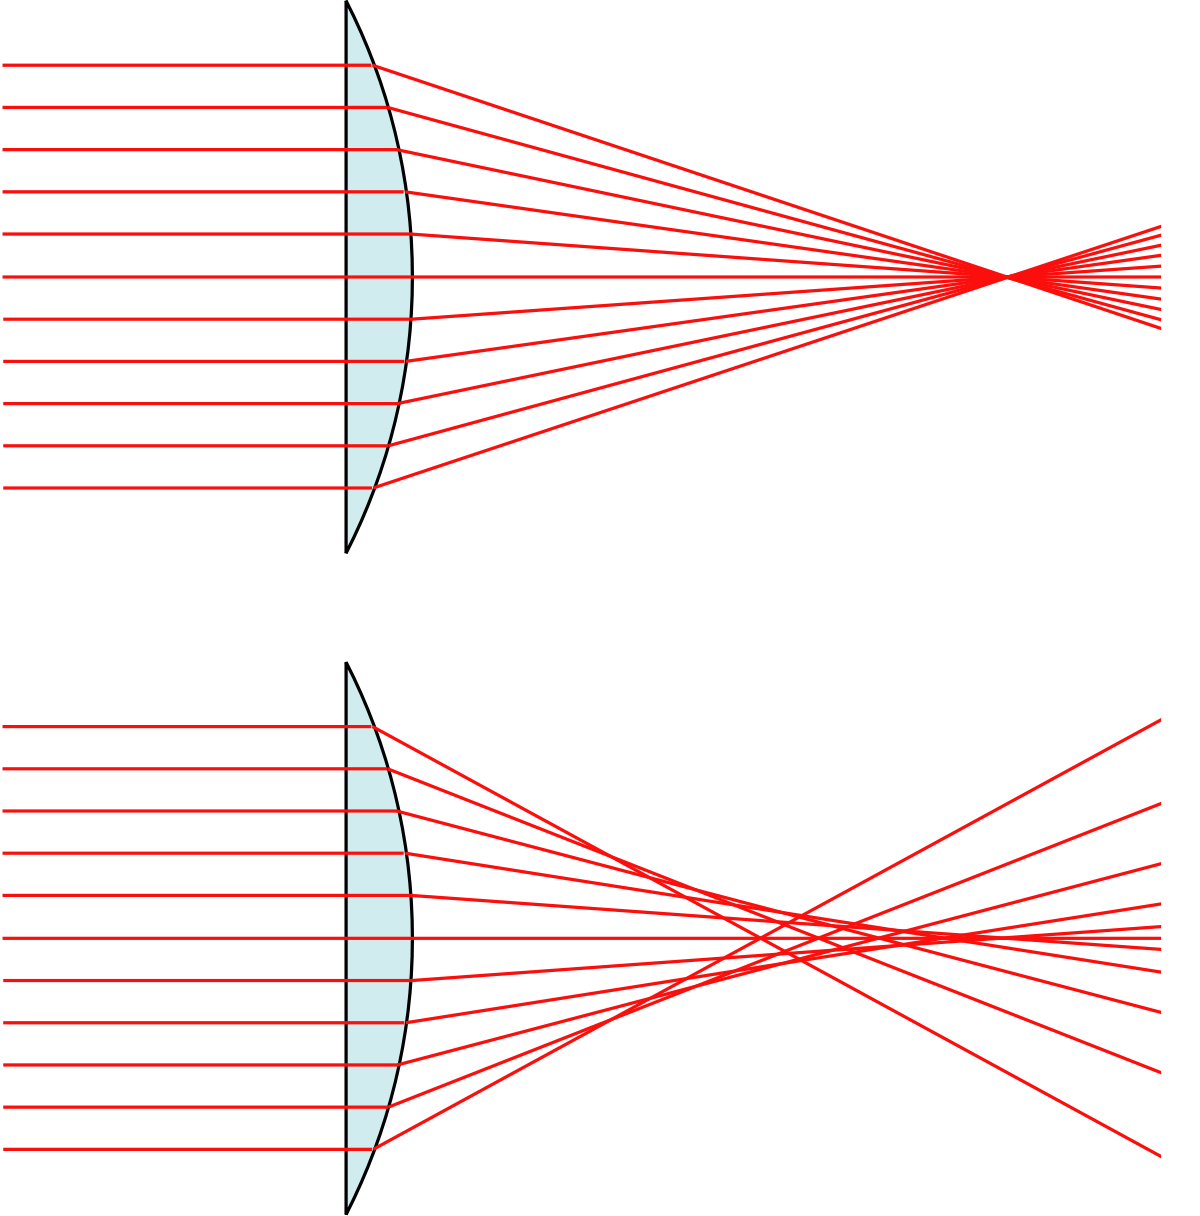
\includegraphics[width=6cm]{obrazky-figures/sphericalAberrationWikipedia.png}
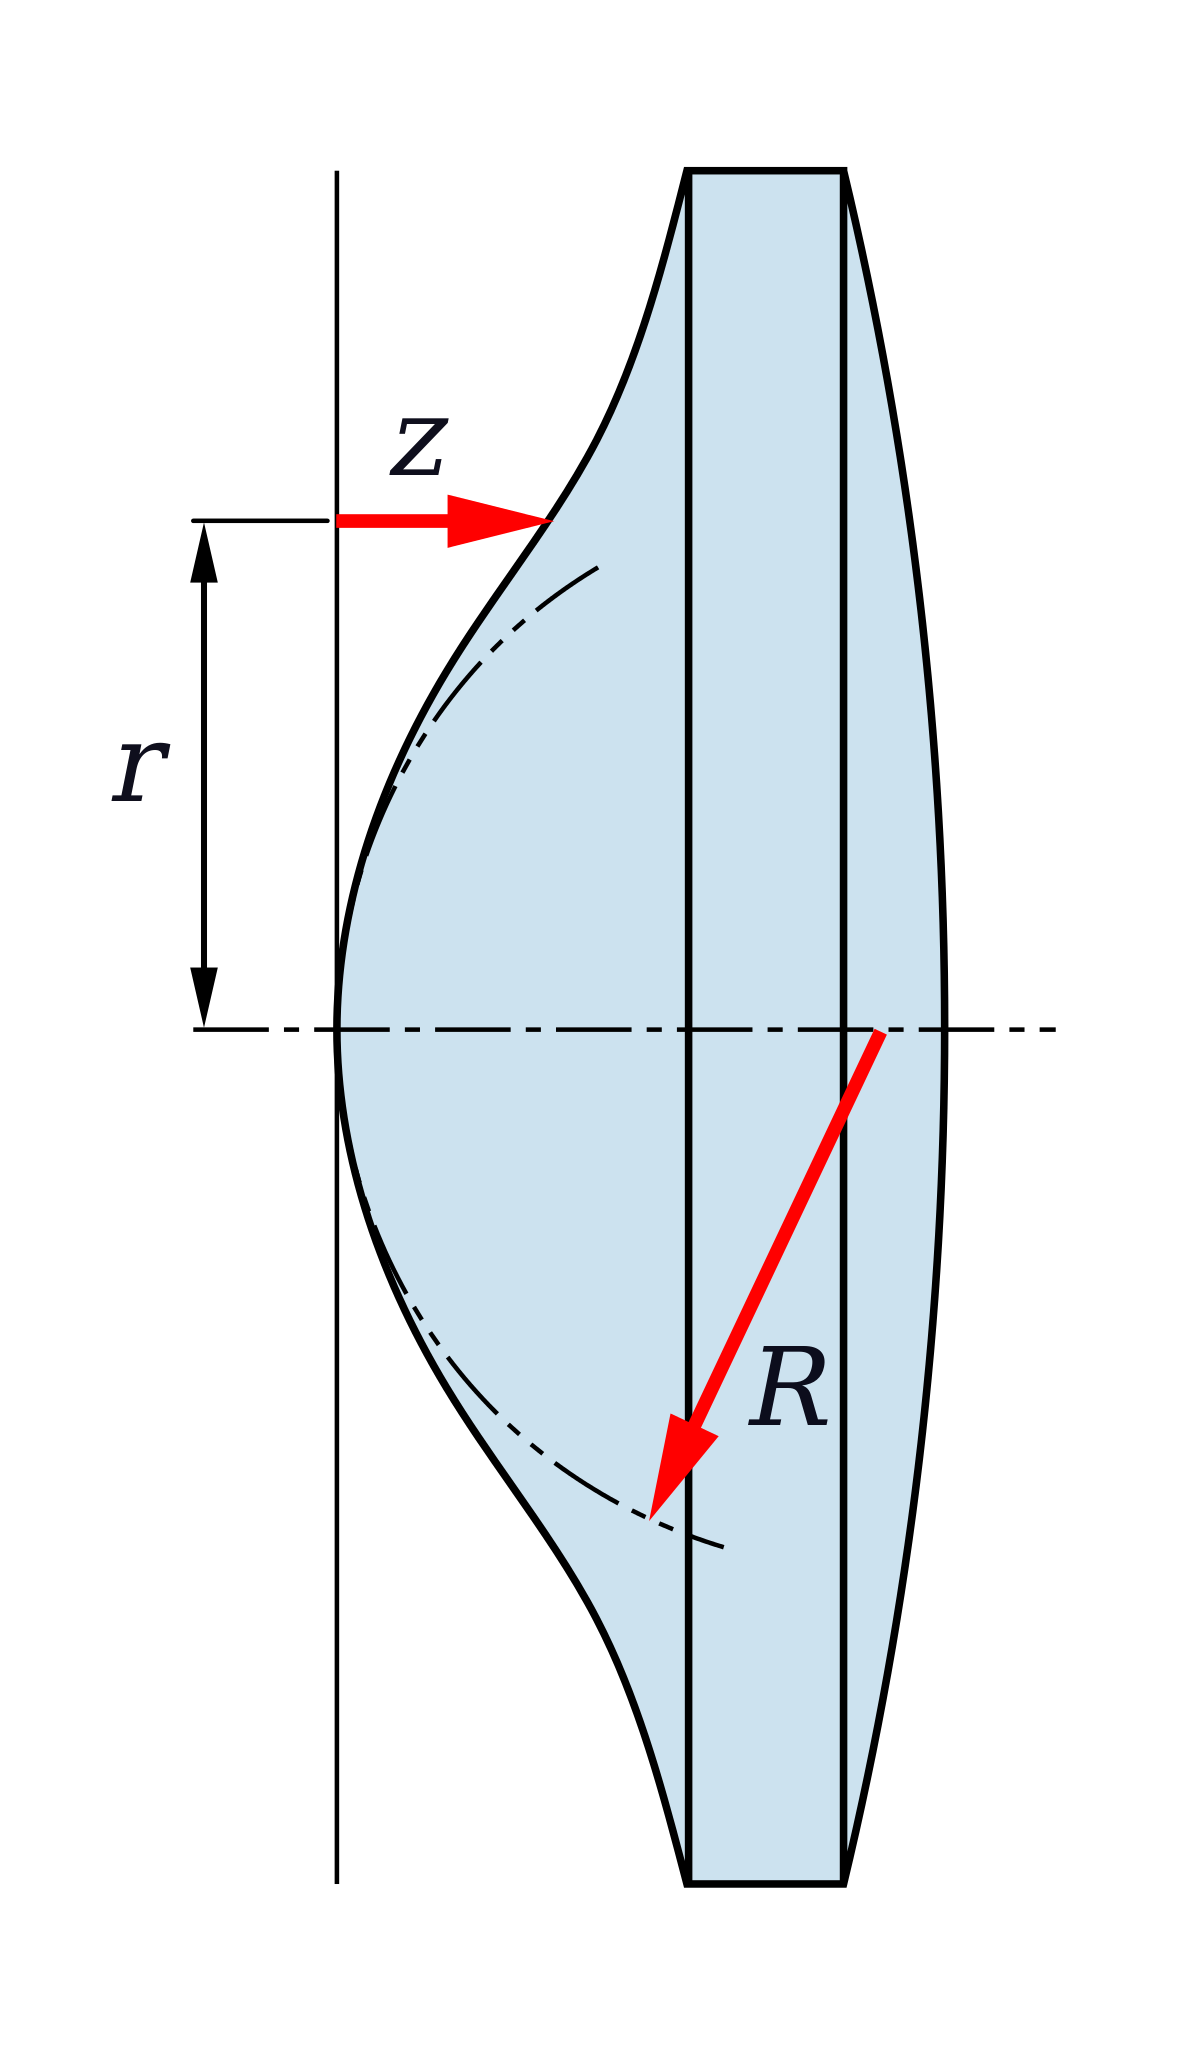
\includegraphics[width=3cm]{obrazky-figures/asphericLen.png}
\caption{Ilustrácia sférickej aberácie. Vplyvom zakrivenia sa ľúče na rozhraní nelámu smerom
    do jedného ohniska. Prevzaté z Wikipédie\cite{sphericalAberrationWiki}.}
\end{figure}

Keďže táto aberácia nastáva pri rovnobežných ľúčoch, týka sa obvykle teleskopov, pri ktorých
pozorované objekty sú tak vzdialené, že vlny, ktoré vysielajú môžeme považovať za rovinné.

Sférickú aberáciu je možné riešiť nahradením sférického tvaru zrkadla za parabolický,
prípadne použitím \textit{asferických šošoviek}, ktoré vďaka svojmu tvaru nepodliehajú tejto
aberácii. Šošovka tohoto tvaru je vyzobrazená na obrázku \ref{saill}. Ďalším riešením
môže byť vloženie prídavného optického prvku, ktorý túto vadu zredukuje. Príkladom môže
byť \textit{Schmidtov korektor}.

\begin{figure}
    \centering
    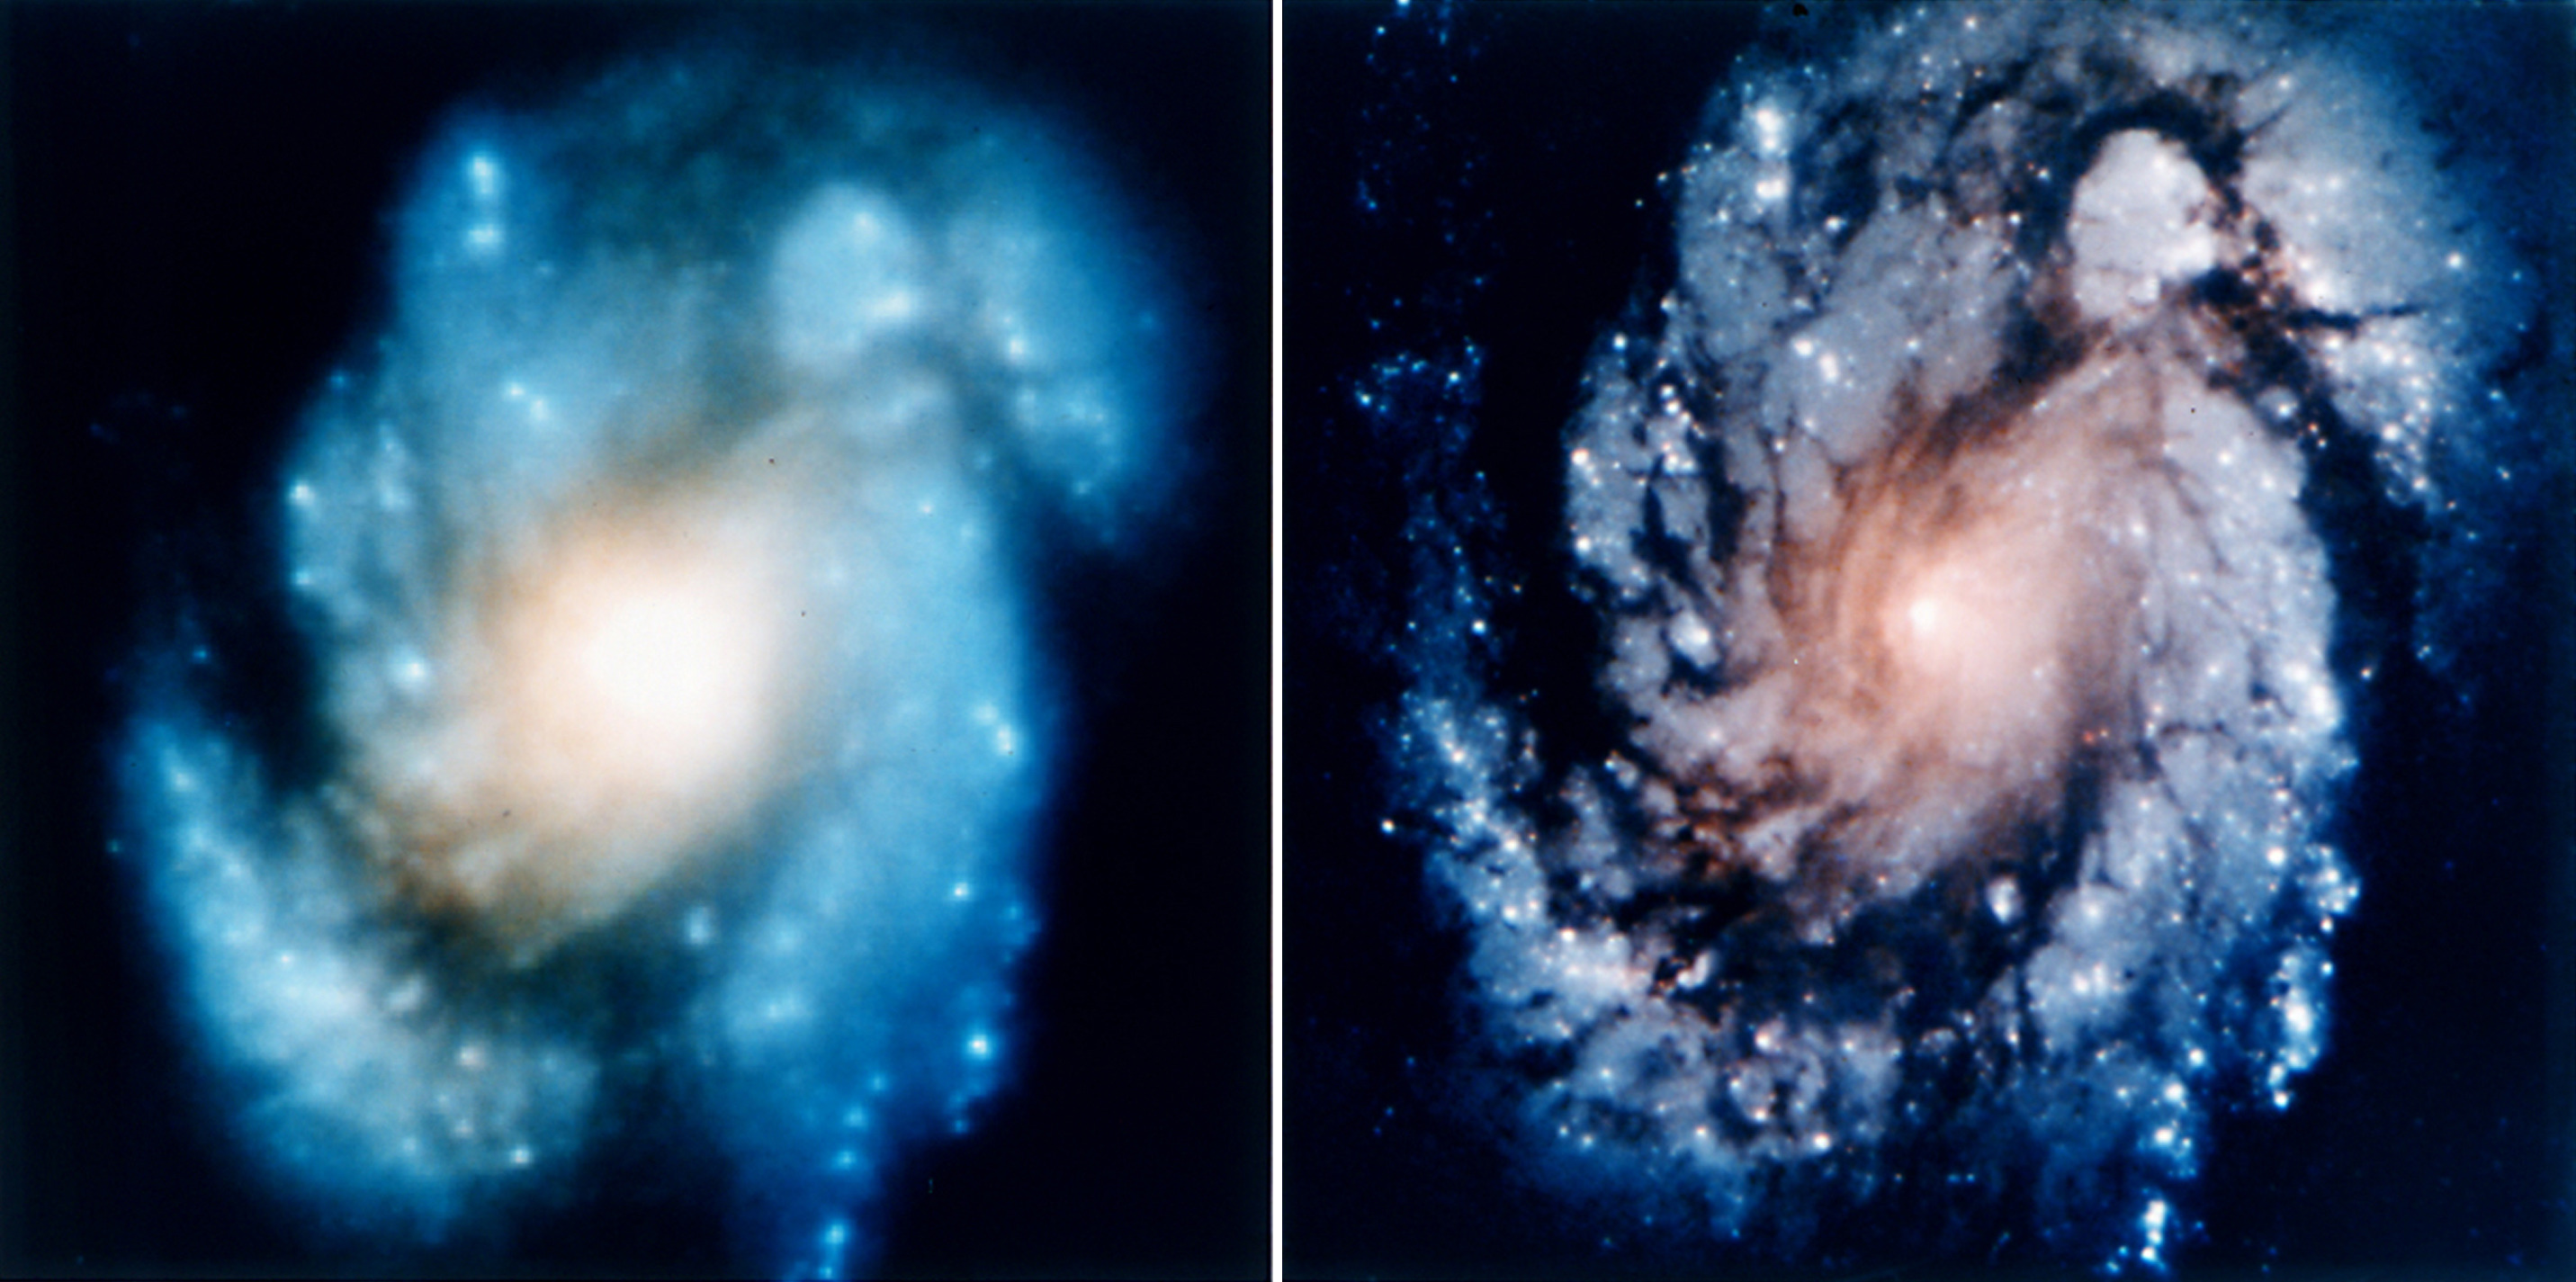
\includegraphics[scale=0.3]{obrazky-figures/costarNASA.png}
    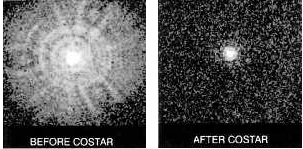
\includegraphics[scale=0.6]{obrazky-figures/cosar.png}
    \caption{Obraz z Hubblovho teleskopu pred a po korekcii. Odstránením sférickej aberácie došlo k
    odstráneniu rozmazania. Zdroj\cite{nasaHubble}}
    \label{hubbleImage}
\end{figure}


Ako praktický príklad dôležitosti odstránenia aberácií môžeme uvažovať \textit{Hubblov vesmírny
teleskop},
ktorý bol vynesený do vesmíru v roku 1990. Krátko po jeho spustení bolo zistené, že obraz
teleskopu nedosahuje predpokladanú kvalitu. Dôvodom degradácie bol tvar hlavného zrkadla, ktoré bolo
príliš ploché, čo spôsobovalo sférickú aberáciu. Problém bol vyriešený pomocou prídavného modulu
\textit{COSTAR}\cite{hechtoptics}. Rozdieľ pred a po aplikácii korekcie je možné pozorovať na obrázku
\ref{hubbleImage}. 

\begin{figure}
    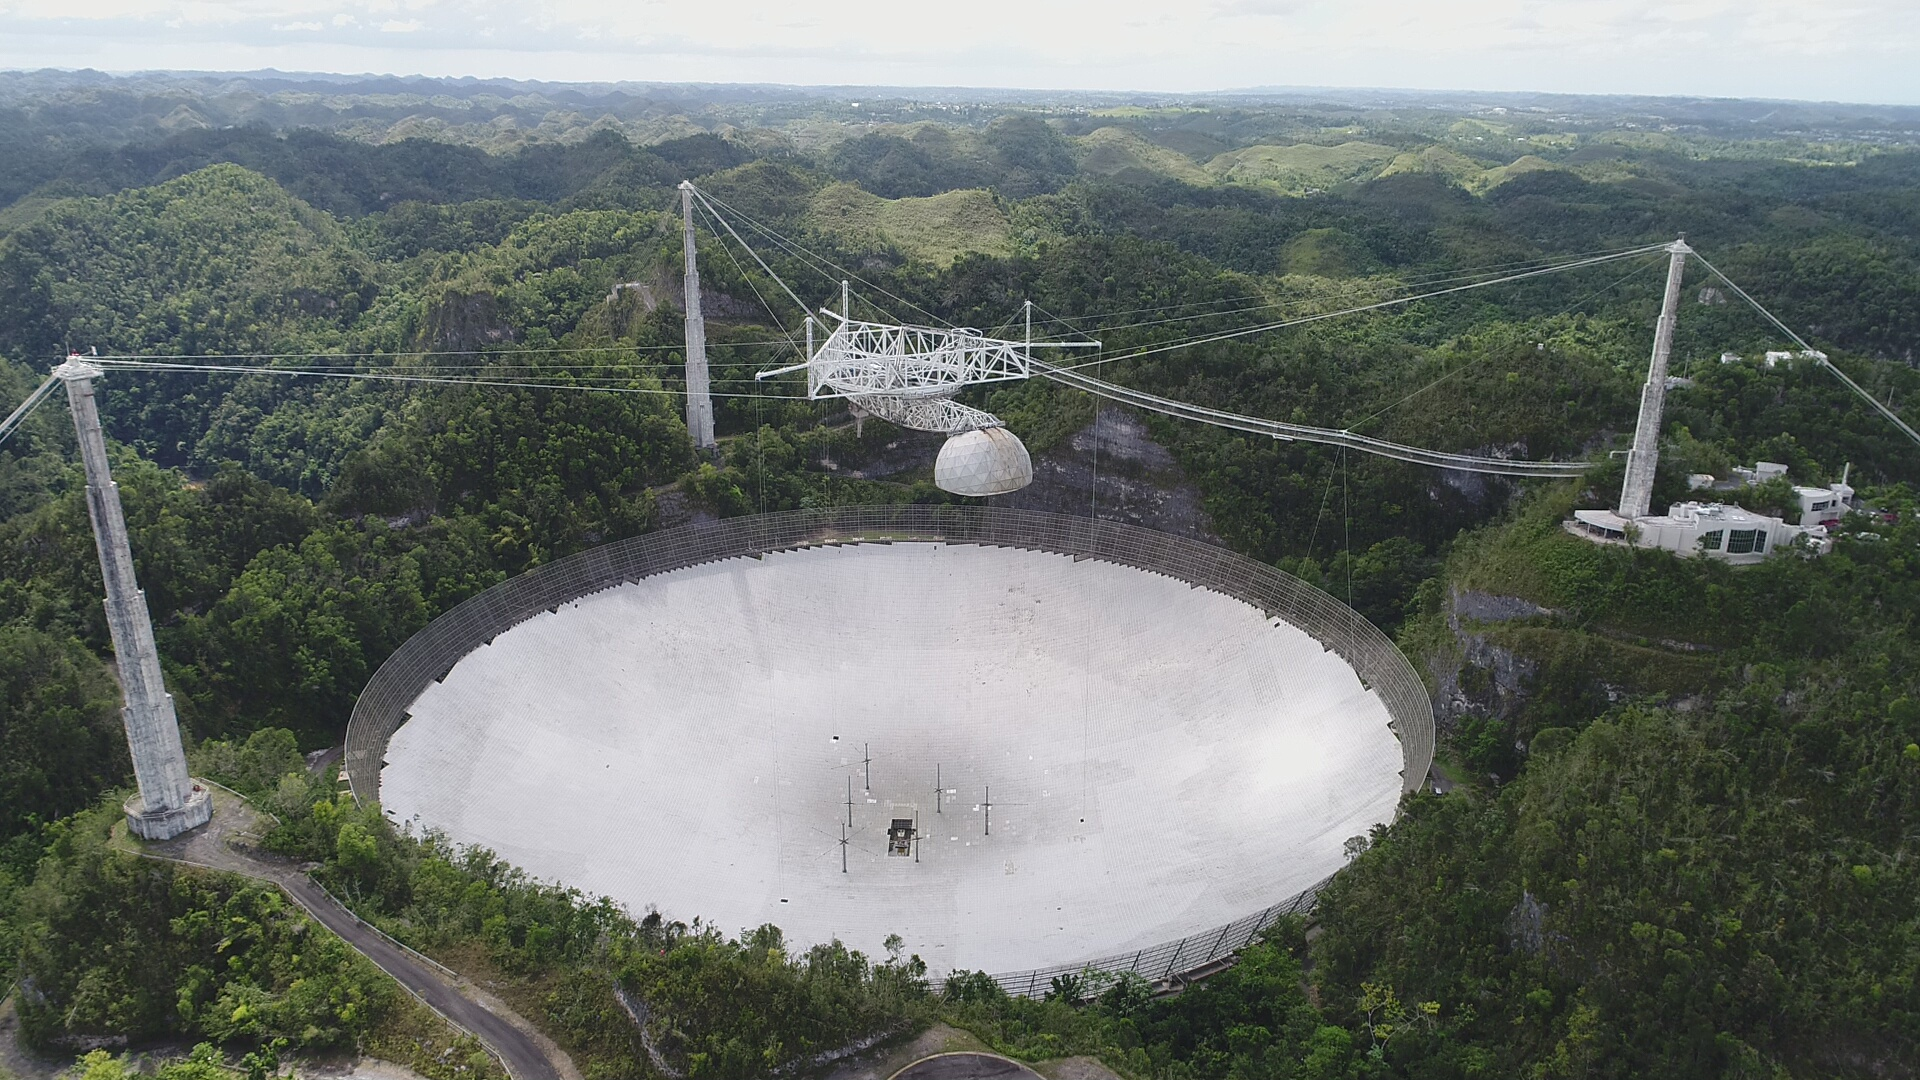
\includegraphics[scale=0.12]{obrazky-figures/areciboSite.jpg}
    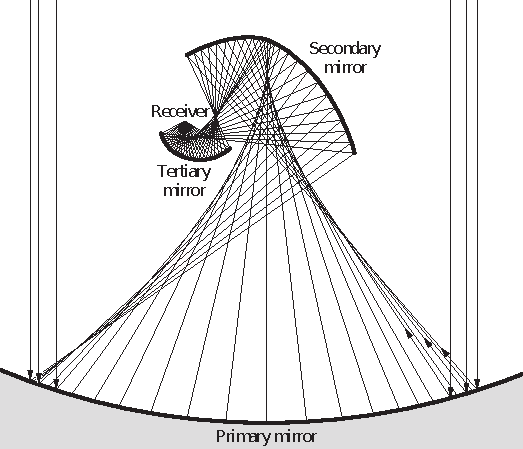
\includegraphics[scale=0.65]{obrazky-figures/arecibo.pdf}
    \caption{Pohľad na prijímač v Arecibo, Puerto Rico. Vpravo schéma optickej sústavy, tvorenej
    primárnym zrkadlom a prijímačom.}
\end{figure}


Ďalším zaujímavým príkladom projektu, ktorý musel ošetriť sférickú aberáciu, je najvačší
radioteleskop na zemi, nachádzajúci sa v Arecibe, Puerto Rico, ktorý je známy z filmu
\textit{GoldenEye} s hlavnou postavou Jamesa Bonda. 
Obvykle majú obdobné observatória zrkadlá v \textit{parabolickom tvare}, ktoré netrpia sférickou
aberáciou, ale musia sa vhodne natáčať podľa smeru záujmu tak, aby ľúče dopadali kolmo. Keďže hlavné zrkadlo tohoto observatória má
zhruba 300 metrov v priemere, z konštrukčných dôvodov bolo navrhnuté ako staticky umiestnené v
teréne, a zároveň
bolo nutné zvoliť sférický tvar aby malo zrkadlo rovnaké vlastnosti z každého smeru.


Z tohoto dôvodu je nad primárnym zrkadlom pohyblivo zavesený 90 ton vážiaci prijímač, ktorý je poziciovaný
podľa smeru záujmu a zároveň obsahuje ďalšie zrkadlá, ktoré korigujú lúče do jediného fokálneho
bodu\cite{hechtoptics}. Detail prijímača je možné pozorovať na obrázku \ref{areciboReceiver}.

\begin{figure}
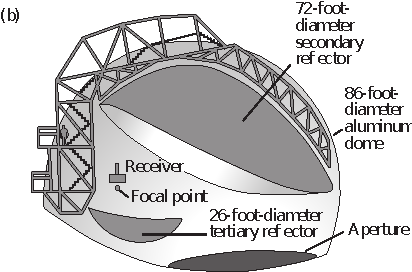
\includegraphics[scale=0.9]{obrazky-figures/areciboReceiver.pdf}
    \centering \caption{Detail prijímača. Ľúče vstupujú cez uzáverku, odrážajú sa od druhotného a
    následne terciálneho zrkadla až do prijímača. Zdroj\cite{hechtoptics}}
\end{figure}

\subsection{Coma}
Ďalšou z aberácii je coma, ktorá sa vyskytuje pri bodových zdrojoch, ležiacich mimo optickej osy. 
V princípe je coma podobná sférickej aberácii - pozorovaný bodový zdroj je tak vzdialený, že jeho
vlny môžeme uvažovať za rovinné pri dopade na rozhranie šošovky, zároveň ale bod leží mimo osy,
preto ľúče dopadajú pod uhlom. Tento druh aberácie sa teda podobne ako pri sférickej aberácii týka
teleskopov.
Ako môžeme vidieť na obrázku \ref{comaDescribe}, jednotlivé ľúče majú pri prechode spojkou 
tendenciu stretnúť v jednej línii, ale nie je v jednom bode. Dôsledkom je potom pri zobrazení bodu rozmazaný typický obraz, ktorého
tvar pripomína kométu, ktorý môžeme vidieť na obrázku \ref{comaDescribe}.
\begin{figure}[h]
    \label{comaDescribe}
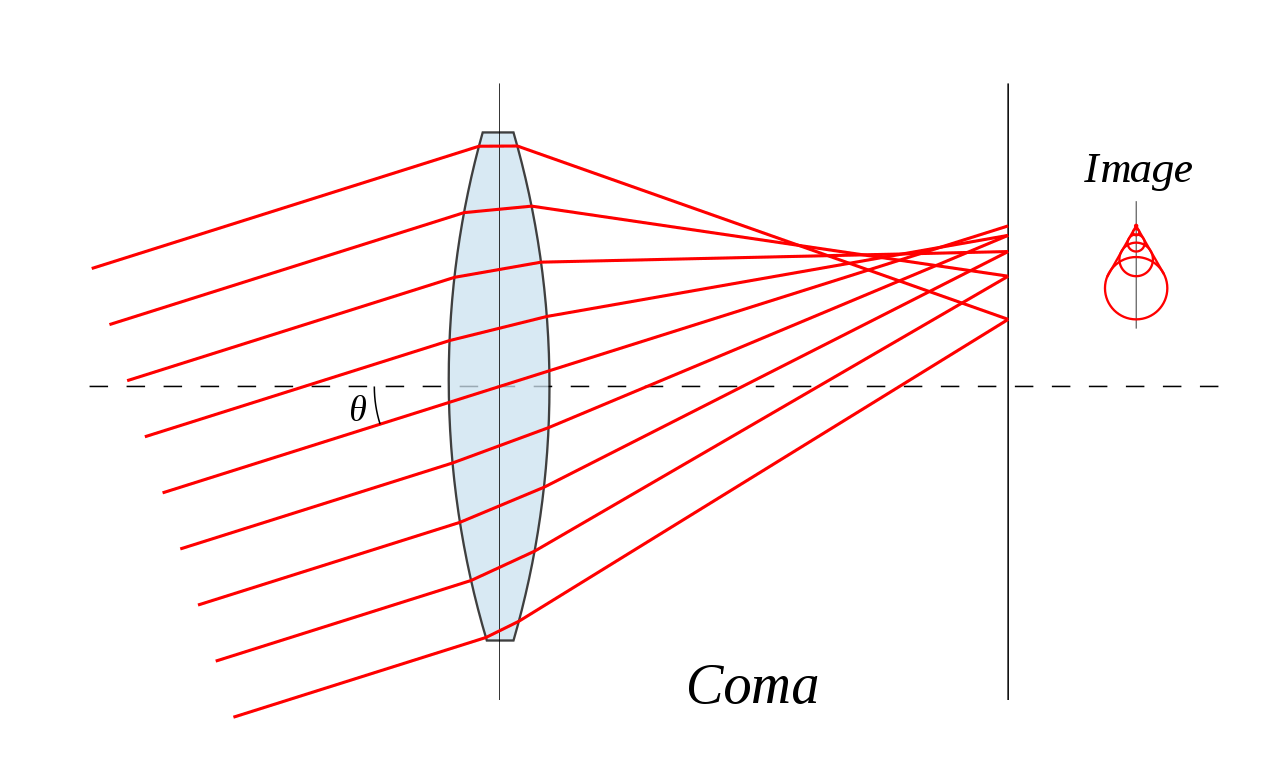
\includegraphics[scale=0.15]{obrazky-figures/coma.png}
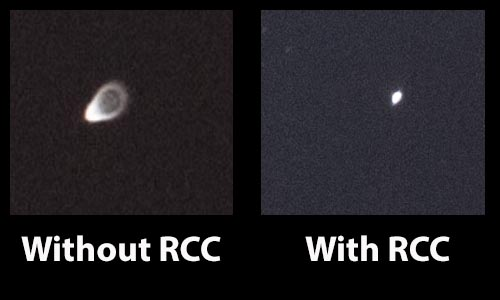
\includegraphics[scale=0.35]{obrazky-figures/coma.jpg}
    \centering \caption{Vľavo: dopad paralelných ľúčov pod uhlom spôsobuje nedokonalý fokus ľúčov v
    obrazovej rovine. Vpravo: príklad obrazu pred a po korekcii comy}
\end{figure}

Efekt comy je možno minimalizovať zmenou krivosti šošovky. Podľa literatury je najvhodnejším tvarom 
konvexne-planárna šošovka \cite{hechtoptics}[str. 272].

Efekt comy je taktiež možné ovplyvniť pridaním \textit{blokovacej apertúry} pred šošovku na vhodné miesto.
Detaily je možné nájsť v literatúre\cite{hechtoptics}.


\subsection{Petzvald field curvature}
Táto aberácia sa týka paralelných ľúčov, dopadajúcich pod rôznymi uhlami. Podľa ideálneho modelu
šošovky by sme očakávali, že tieto ľúče budú mať ohnisko v rovnakej vzdialenosti od šošovky. 
V skutočnosti je ohnisko závislé na uhlu dopadu a pozícia jednotlivých ohnísk bude sledovať tvar
krivky, čo môžeme pozorovať na obrázku \ref{comaDescribe}.

Dôsledkom tejto aberácie je fakt, že obraz nie je možné zachytiť rovinou bez vzniku rozmazania. 
Príkladom kompenzácie tejto vady môže byť pole senzorov z \textit{Keplerovho versmírneho teleskopu},
ktorých rozloženie nie je rovinné, ale zakrivené.

\begin{figure}[h]
    \label{comaDescribe}
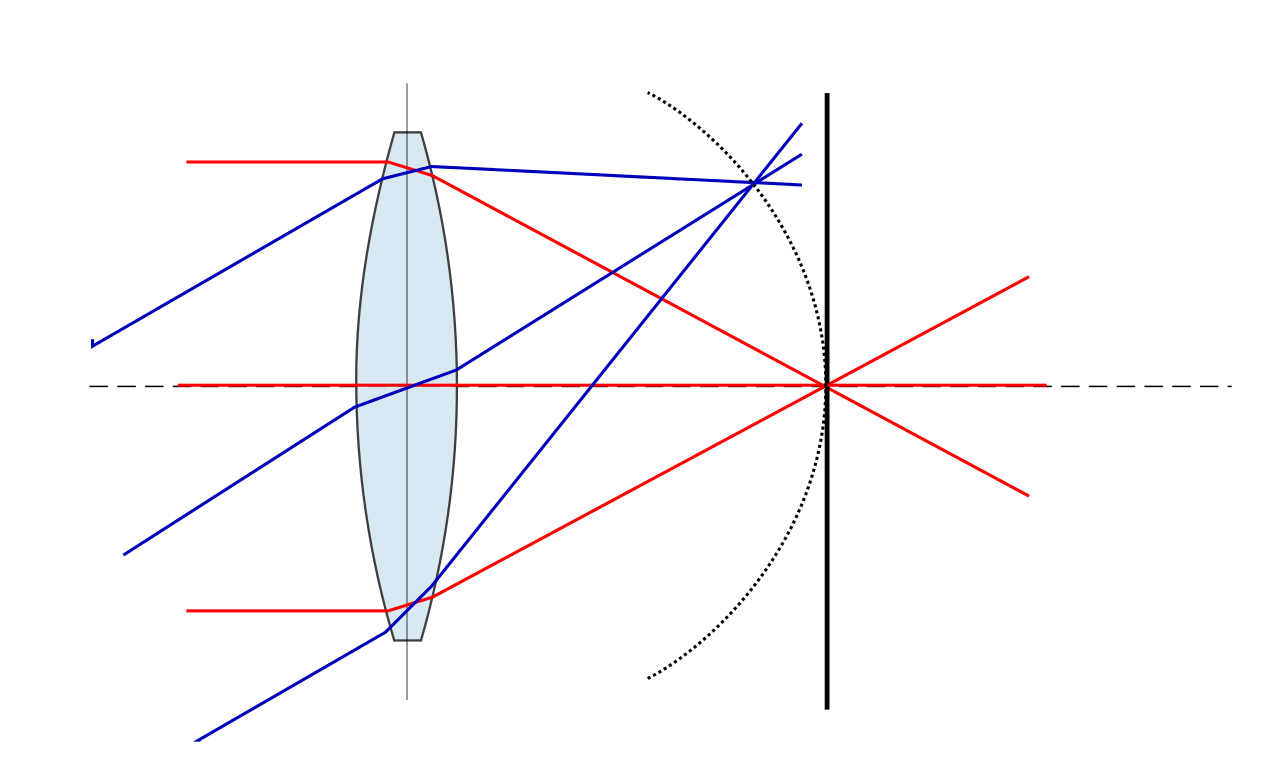
\includegraphics[scale=0.15]{obrazky-figures/fieldcurvature.png}
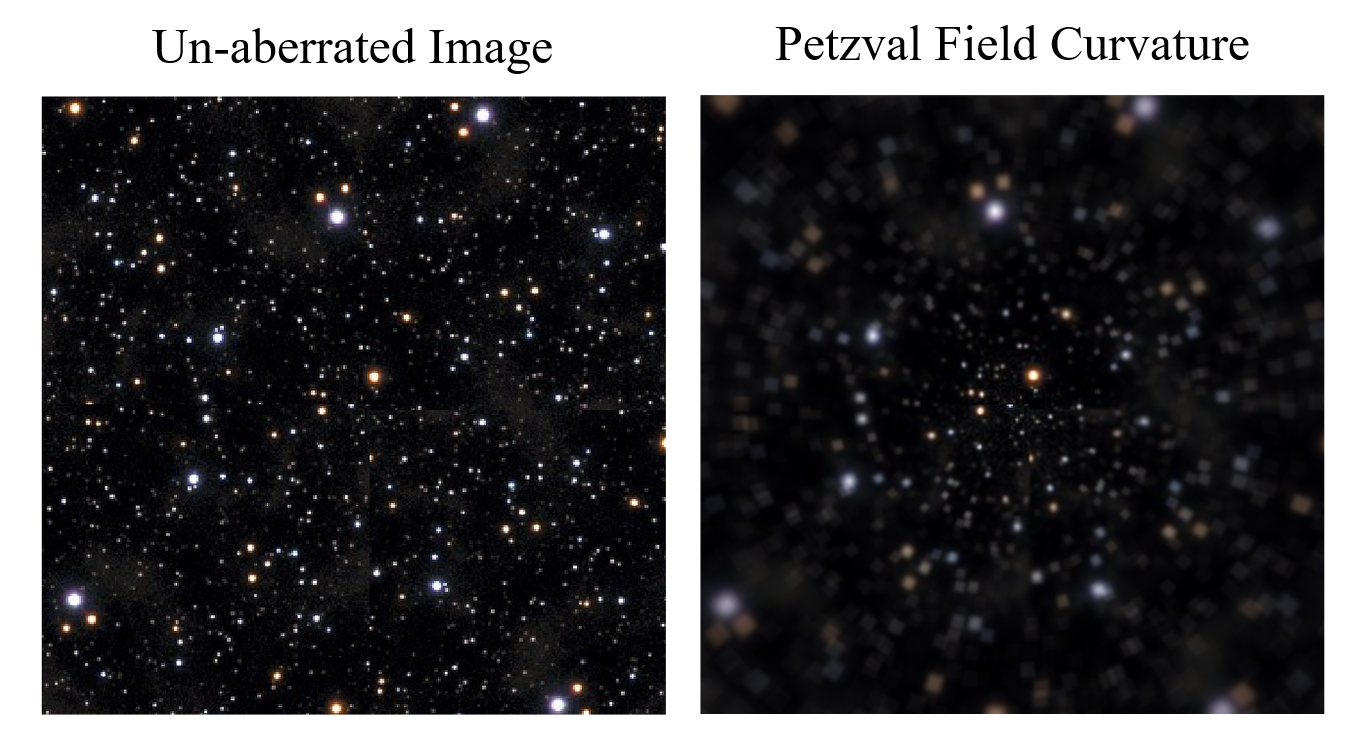
\includegraphics[scale=0.60]{obrazky-figures/fieldAberration.png}
    \centering \caption{Vľavo: }
\end{figure}



\subsection{Astigmatizmus}

Astigmatizmus sa môže vyskytovať aj v ľudskom oku z dôvodu nedokonalosti šošovky. Vizuálny prejav
astigmatizmu je znázornený na obrázku \ref{comaDescribe}.

\begin{figure}[h]
    \label{comaDescribe}
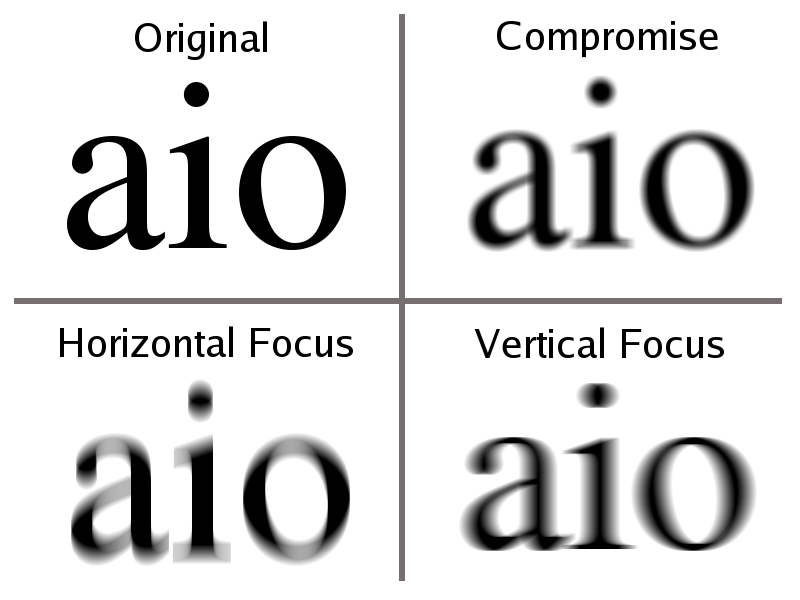
\includegraphics[scale=0.30]{obrazky-figures/astigmatism.png}
    \centering \caption{Demonštrácia vizuálneho astigmatizu, teda vnemu, akým vnímajú obraz osoby,
    trpiace touto chorobou.}
\end{figure}



\section{Chromatická aberácia}
Chromatická aberácia je jav šošovky, kedy jednotlivé vlnové dĺžky sú odlišne lomené pri dopade na
rozhranie šošovky. Dôsledkom toho je posunutie ohniska jednotlivých farebných zložiek v obraze, ktoré je
znázornené na obrázku \ref{chromaticFocus}. 

\begin{figure}[h]
\centering
\label{chromaticFocus}
%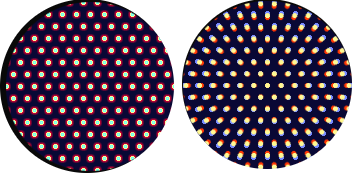
\includegraphics[width=6cm]{obrazky-figures/chromaticAberrationDifference.png}
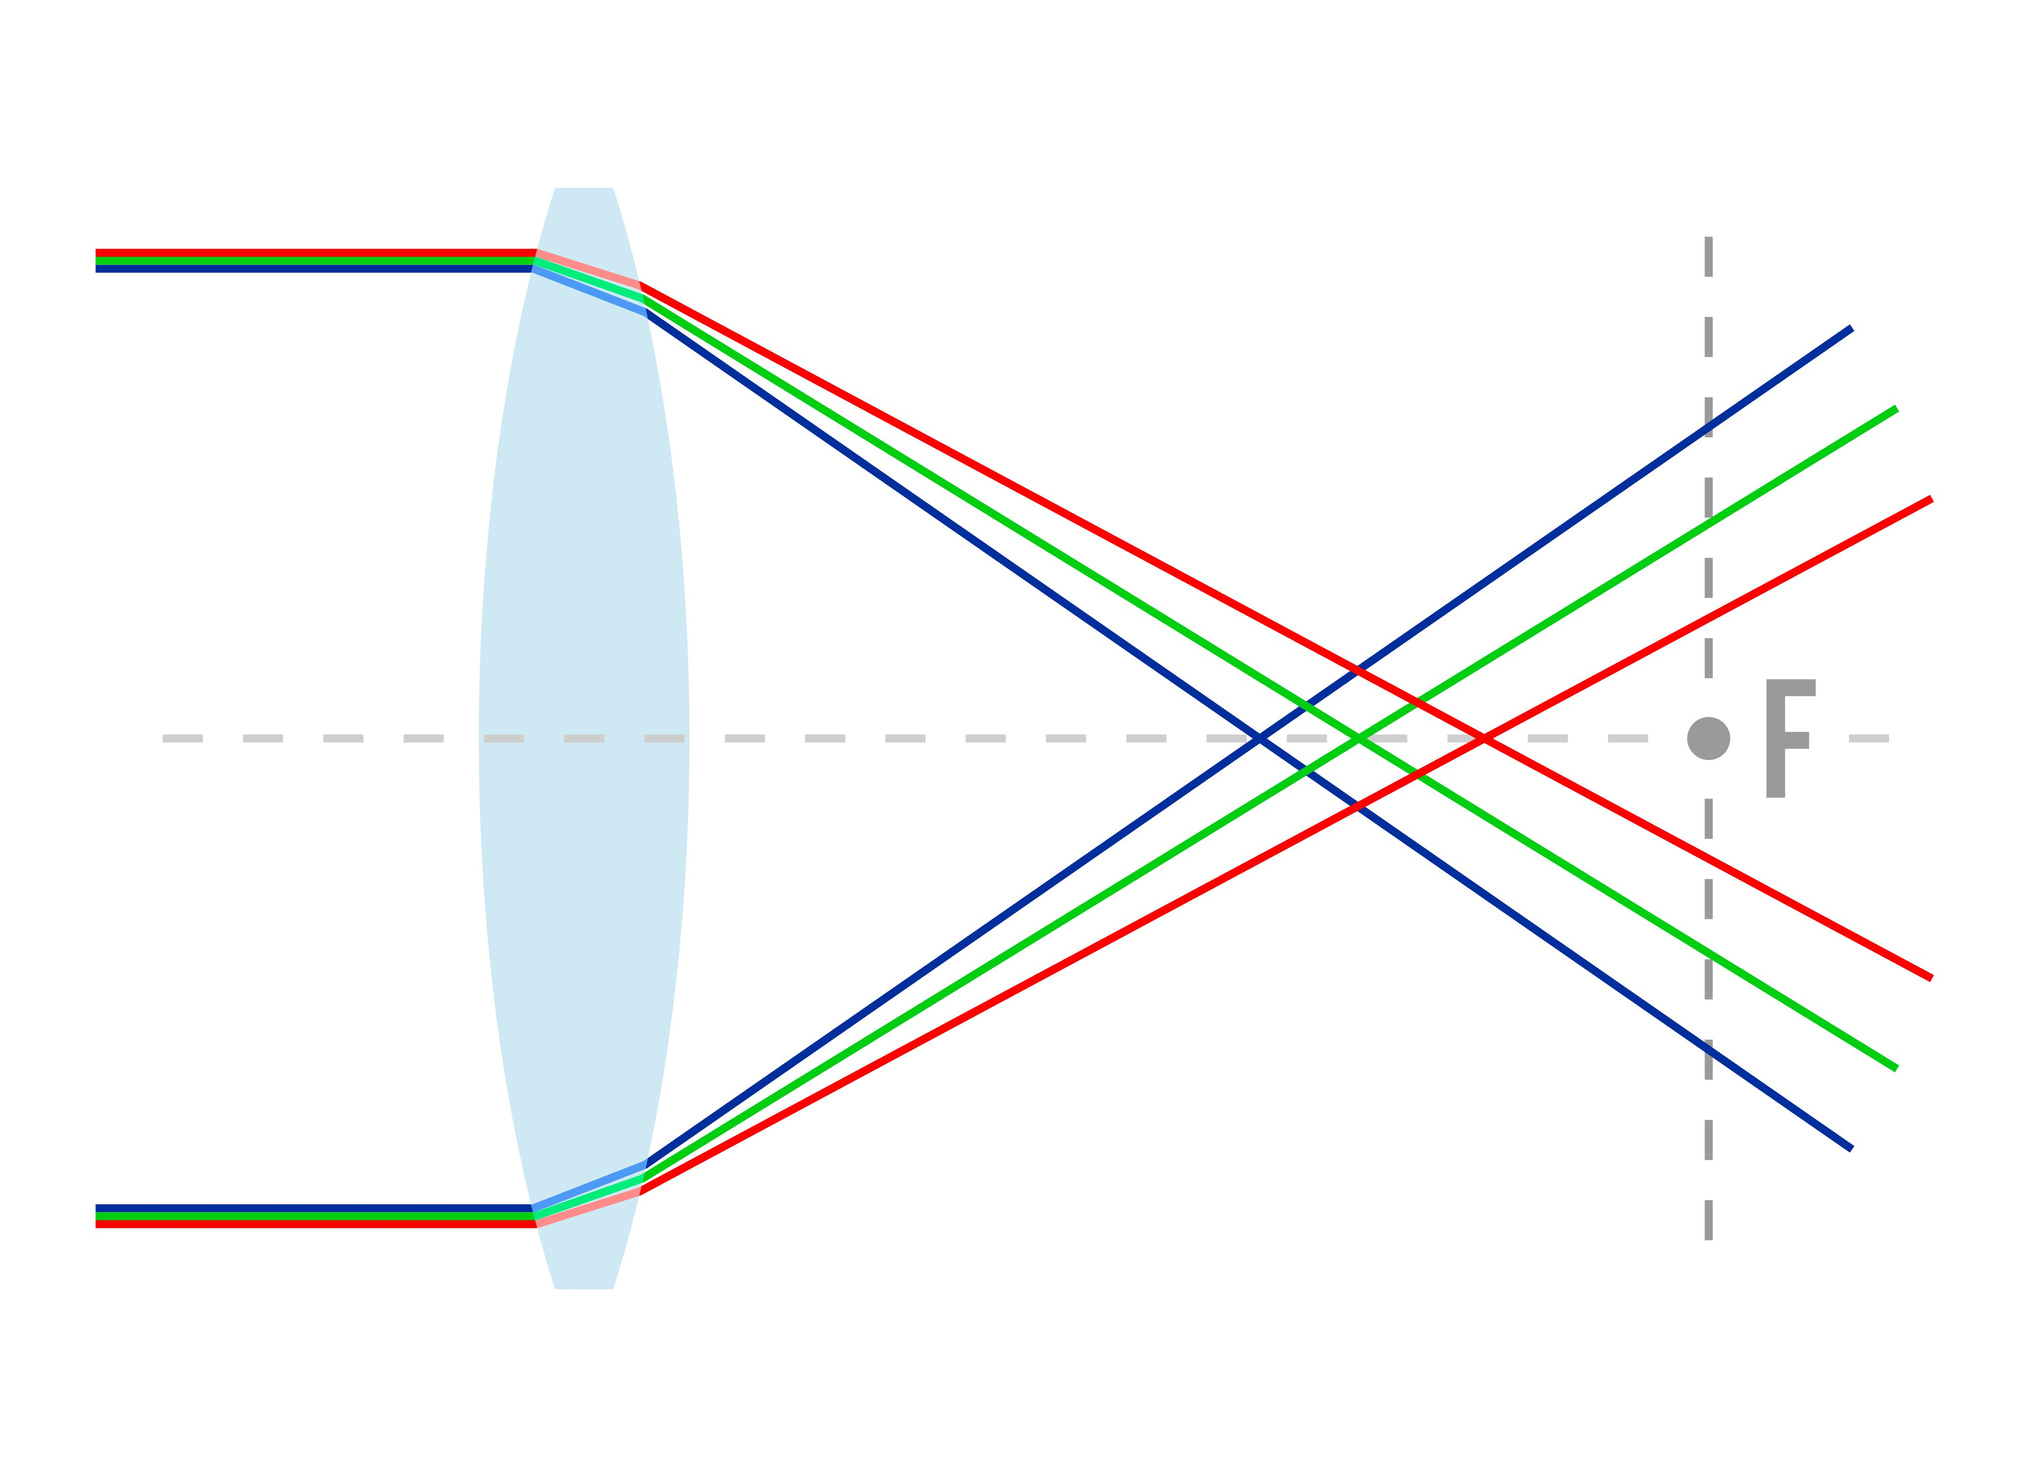
\includegraphics[width=6cm]{obrazky-figures/chromaticFocus.jpg}
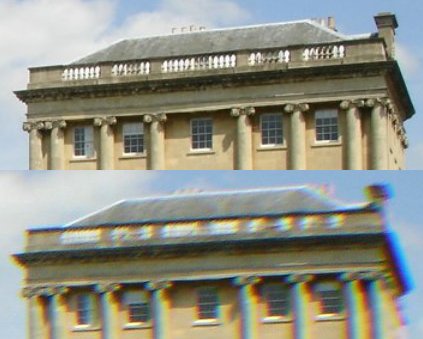
\includegraphics[width=6cm]{obrazky-figures/chromaticAberrationWikipedia.jpg}
\caption{Vlavo: pre ľúče rôznej vlnovej dĺžky nastáva posun ohniska vplyvom rôzneho indexu lomu. Vpravo:
   jednotlivé farebné zložky sú v obraze posunuté v dôsledku priečnej chromatickej aberácie.}
\end{figure}

V prípade, že lúče dopadajú rovnobežne, hovoríme o
\textit{dĺžkovej chromatickej aberácii}, ktorá posúva ohniská jednotlivých vlnových dĺžok pozdĺž optickej
osy. Ak ale ľúče dopadajú na rozhranie pod uhlom, nastáva priečne posunutie ohnísk, čo je označované
ako \textit{priečna chromatická aberácia}. Rozdieľ oboch typov aberácii je znázornený na obrázku
\ref{chromaticDifference}.

Chromatická aberácia je variáciou známejšieho javu, ktorým je \textit{disperzia svetla}.
Príčinou tejto aberácie je fakt, že index lomu prostredia je funkciou vlnovej dĺžky, preto výsledný
uhol lom je závislý na vlnovej dĺžke. Samotná variácia indexu lomu v závislosti na vlnovej dĺžke nie
je fixná, ale líši sa pre konkrétne materiály. Obrázok \ref{chromaticDifference} ukazuje príkladnú
tabulku, udávajúcu hodnoty koeficientov indexu lomu konkrétneho typu skla pre rozličné vlnové dĺžky.

\begin{figure}[h]
\centering
\label{chromaticDifference}
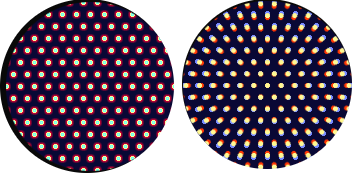
\includegraphics[width=6cm]{obrazky-figures/chromaticAberrationDifference.png}
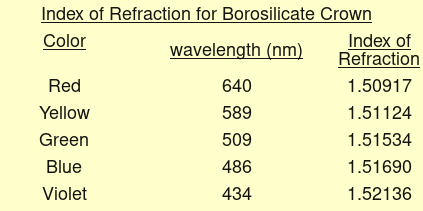
\includegraphics[width=6cm]{obrazky-figures/chromaticRefraction.png}
\caption{Vlavo dĺžková, vpravo priečna chromatická aberácia a jej dôsledok na výsledný obraz.
    Zdroj\cite{chromaticAberrationsAstro}. Vpravo tabuľka, udávajúca index lomu pre jednotlivé
    vlnové dĺžky v borosilikátovom skle.}
\end{figure}

Chromatickú aberáciu je možné riešiť niekoľkými spôsobmi. Triviálne riešenie spočíva v nahradení
lomivého optického prvku za odrazivý, nakoľko odraz nie je závyslý na vlnovej dĺžke \cite[elert]. 
Iné riešenie pozostáva vo vytvorení obrazu tromi nezávyslými optickými sústavami, ktoré by boli
vyľadené na konkrétnu vlnovú dĺžku, a následnou kompozíciou obrazu \cite{automaticRemovalCA}. Toto riešenie ale bude
dostatočné len pre statické scény.

Z hľadiska optiky je možné použiť \textit{achromatické šošovky}, ktoré sú vyrobené kombináciou dvoch
rôznych materiálov za cieľom minimalizovania tejto aberácie. Tento spôsob ju ale nedokáže úplne 
odstrániť pre všetky vlnové dĺźky, pretože závislosť indexu lomu obvykle nie je lineárna na vlnovej
dĺžke\cite{chromaticFix}.

Nakoniec, pre riešenie chromatickej aberácie existuje niekoľko algoritmov, ktoré dokážu utlmiť
prejavy aberácie v existujúcom digitálnom obraze. Tieto riešenia napríklad realizujú tzv.
\textit{warping} jednotlivých farebných zložiek obrazu tak, aby sa detekované hrany v obraze
prekrývali \ref{automaticRemovalCA}.

\section{Demonštračný projekt}
Vrámci tejto práce bol vypracovaný programový projekt, ktorého cieľom bolo umožňiť uživateľovi
experimentovať s ľúčovou optikou a zároveň sa zoznámiť s vybranými aberáciami.

Projekt bol implementovaný v jazyku \textit{Javascript} pomocou knižnice \textit{PIXI.js} pre prácu
s HTML plátnom. Jeho jadrom je vykreslovanie dráhy ľúčov, ktoré postupujú z ľava do prava. 

Projekt umožňuje uživateľovi nastavovať pozíciu a krivosť spojky, zároveň nastavovať typ zdroja 
ľúčov, ako aj ich množstvo a výškové obmedzenie. Vzhľadom na rozsiahly počet parametrov aplikácie
boli vybrané vhodné konfigurácie, ktoré demonštrujú jednotlivé aberácie.

\begin{figure}
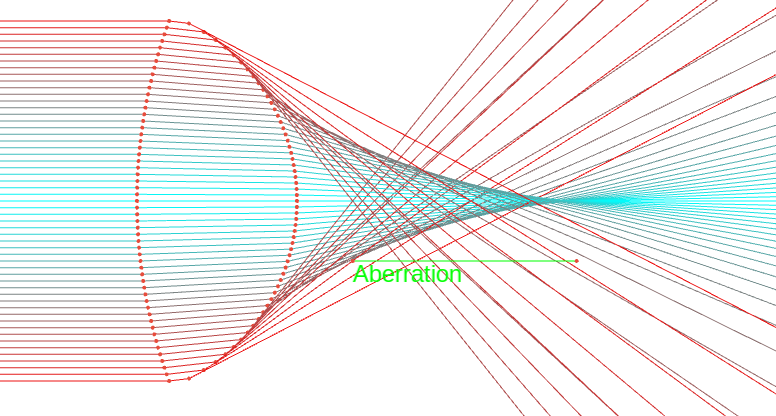
\includegraphics[scale=0.4]{obrazky-figures/application.png}
    \centering \caption{Príkladný výstup, ktorý uvidí uživateľ aplikácie pri konfigurácii sférickej aberácie.}
\end{figure}

\section{Záver}
V texte práce boli predstavené základné aberácie šošoviek, konkrétne sférická aberácia, coma,
astigmatizmus, Petzvaldovo zakrivenie poľa a chromatická aberácia.




